\documentclass{beamer}

\usetheme{Madrid}

\usepackage{graphicx}
\usepackage{amsmath}



\title[Necessary Conditions of Political Unification]{External Threats, Linguistic Homogeneity, and Political Unification}
\author{Chen Zeng}
\institute[]{Department of Political Science \\ Renmin University of China}

\begin{document}
	\maketitle
	\begin{frame}{Introduction}
		\begin{columns}
			\begin{column}{.4\textwidth}
				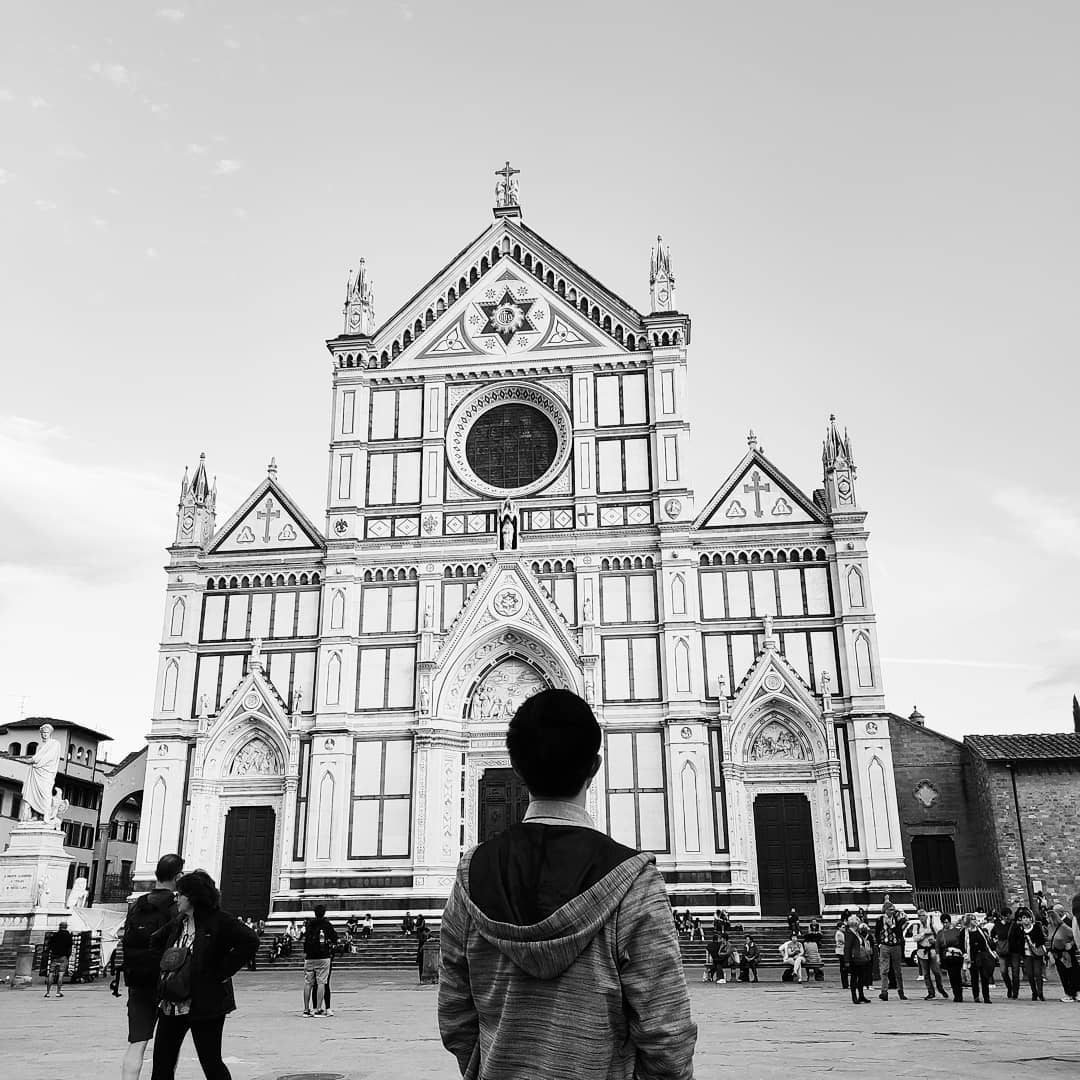
\includegraphics[width=\textwidth]{santa_croce.jpg}
			\end{column}
			\begin{column}{.6\textwidth}
				Niccolò Machiavelli, a Florentine in the 16th century, argued for the unification of Italy, which didn't happen until the \textit{Risorgimento} in 19th century, citing the following reasons:
				\begin{itemize}
					\item Florentine lifestyle
					\item The Italian language, i.e. Tuscan dialect
					\item Women, god, and heroes
					\item External interference
				\end{itemize}
				Today we look at two key elements in the political unification of states --- external security threats and linguistic homogeneity.
			\end{column}
		\end{columns}
	\end{frame}
	\begin{frame}{Contents}
		\tableofcontents
	\end{frame}
	\section{Conceptualization and Operationalization}
	\subsection{Political Unification}
	\begin{frame}{Political Unification}
		\begin{block}{Definition}
			\begin{description}
				\item[Political unification] occurs when two or more sovereign states merge into one.
			\end{description}
		\end{block}
		\begin{itemize}
			\item Political unification has been one of the most debated areas in the study of political science.
			\item Notable instances included the US (American Revolutionary War), Germany (\textit{Sonderweg}), and Italy (\textit{Risorgimento}).
			\item Does the unification happen incrementally, or is there a clear moment for such unification?
			\item Recent development of the EU, free trade areas, and customs unions has led political scientists to examine if there are limits to such political and economic integration. To which point do they stop being just ``integration'' and become unification?
		\end{itemize}
	\end{frame}
	\begin{frame}{Political Unification}
		\begin{itemize}
			\item An \textit{operational} definition of political unification used in this article is that two sovereign states voluntarily merge into a federation or unitary state. Conquests/accessions are excluded.
			\begin{description}
				\item[Unit of analysis] Political unification (of a state dyad)
				\item[Unit of observation] Inter-state actions (dichotomous variable: unification, linguistic homogeneity); and individual states (continuous variable: threat levels)
			\end{description}
		\end{itemize}

		\begin{itemize}
			\item This research leverages datasets from the Correlates of War project. Qualifying states have to meet at least one of the following criteria.
			\begin{description}
				\item[Criterion 1] Before 1920, a population of at least 500,000 and establishment of diplomatic missions at or above the rank of \textit{chargé d'affaires} by Britain and France.
				\item[Criterion 2] After 1920, membership in the League of Nations or United Nations \textit{or} a population of at least 500,000 and establishment of diplomatic missions from any two major powers.
			\end{description}
		\end{itemize}
	\end{frame}

	\begin{frame}{Research Hypotheses}
		\begin{description}
			\item[Hypothesis 1] External threats are \textit{necessary} for political unification.
			\item[Hypothesis 2] Linguistic homogeneity is \textit{necessary} for political unification.
		\end{description}
		\begin{itemize}
			\item The article takes on the form of a \textit{falsification} probe and focuses on only \textit{necessary} conditions for political unification.
			\item That is to say that security threats or linguistic homogeneity may not be \textit{sufficient} for political unification, but the lack of either condition cannot result in the expected outcome.
			\item This method is prone to many methodological and substantive vulnerabilities. We will cover them in the final section, but now, let's take a look into why the author sets those two key explanatory variables.
		\end{itemize}
	\end{frame}



	\subsection{External Security Threats}
	\begin{frame}{External Security Threats}
		\begin{itemize}
			\item Riker (1975) argues that states unify for security reasons; they desire protection from external threats
		\end{itemize}
	\end{frame}
	\subsection{Linguistic Homogeneity}
	\section{Exploratory Analysis and Causal Inference}
	\begin{frame}{}
		hi
	\end{frame}
	\section{Reflections}
	\begin{frame}{Reflections}
		In the following subsections, we set let \textit{U} denote political unification, \textit{S} external security threats, and \textit{L} linguistic homogeneity.
		\begin{itemize}
			\item From previous analysis, the author detected 12 cases of political unification from the MID dataset, where linguistic homogeneity is present in all cases. Incorporating the Switzerland case as an outlier, we have 13 cases in total. Mathematically, we have
			\begin{equation}
				P(L|U)=\frac{12}{13} \approx 0.92
			\end{equation}
			\item According to Bayes theorem, we have 
			\begin{equation}
				P(U|L)=\frac{P(U)P(L|U)}{P(L)}
			\end{equation}
		\end{itemize}
	\end{frame}
	\begin{frame}{Reflections}
		\begin{itemize}
			\item Since $P(U)$ and $P(L)$ have the same denominator, we can simplify the equation as
			\begin{equation}
				P(U|L)=\frac{N(U)P(L|U)}{N(L)}
			\end{equation}
			whereas $N(U)=12$, as per previous discussion.
			\item Only considering all 6 UN official languages, we have
			\begin{equation}
%				EN: 19, ES: 20, FR: 29, RU: 5, AR: 22, ZH: 2
				\begin{aligned}
					N(L)< & N(EN)^2 + N(ES)^2 + N(FR)^2 + N(ZH)^2 + \\
					& N(RU)^2 + N(AR)^2 = 2115
				\end{aligned}
			\end{equation}
			\item Furthermore, we calculate the probability of political unification given the presence of linguistic homogeneity.
			\begin{equation}
				P(U|L)=\frac{N(U)P(L|U)}{N(L)}<\frac{12\times 0.92}{2115}\approx 0.52\%
			\end{equation}
		\end{itemize}
	\end{frame}
	\subsection{The Fundamental Problem of Causal Inference}
	\subsection{Selection Bias}
	\begin{frame}{Selection bias}
		hi
	\end{frame}
	\subsection{Confounding Factors -- Geographical Proximity}
	\begin{frame}{Confounding factors -- geographical proximity}
		$x \sim \mathcal{N}(\mu,\,\sigma^{2})$
	\end{frame}
	\subsection{Alternative Research Design -- fsQCA \& Logistic Regression}
	\begin{frame}{Alternative research design -- fsQCA}
		$x \sim \mathcal{N}(\mu,\,\sigma^{2})$
	\end{frame}
	\begin{frame}{Alternative research design -- Logistic Regression}
		\begin{equation}
			logit(P(U))=\beta_0 + \beta_1 \times S + \beta_2 \times L
		\end{equation}
		\begin{equation}
			logit(P(U))=\beta_0 + \beta_1 \times S + \beta_2 \times L + \beta_3 \times S \times L
		\end{equation}
	\end{frame}
\end{document}
